\documentclass[12pt]{article}
\usepackage{fullpage,enumitem,amsmath,amssymb,graphicx}
\usepackage{graphicx} % This is a package for including graphics in your solution.
\usepackage{listings}
\usepackage[final]{pdfpages}


\begin{document}

\begin{center}
{\Large CS168 Spring Assignment 1}

\begin{tabular}{rl}
SUNet ID(s): 05794739 & \\
Name(s): & Luis A. Perez \\
Collaborators: &
\end{tabular}
\end{center}

By turning in this assignment, I agree by the Stanford honor code and declare
that all of this is my own work.

\section*{Part 1}

\begin{enumerate}[label=(\alph*)]
  \item
    Before running the strategies above, we suspect the following will occur. 

    We expect that Strategy 3 will have a lower maximum value than Strategy 2, which in turn has a lower maximum value than Strategy 1 (this seems rather straight forward, given the fact that Strategy 2 can pick from two buckets and Strategy 3 from three).

    As for Strategy 4, it's quite similar to Strategy 2 except it should be worse (higher return value).

    The code for each strategy is below.
    \begin{verbatim}
def strategy1(N: int) -> int:
  binIdxSamples = np.random.randint(low=0, high=N, size=N)
  bins = collections.Counter(binIdxSamples)
  return max(bins.items(), key=lambda x: x[1])[1]

def strategy2(N: int) -> int:
  firstIdx = np.random.randint(low=0, high=N, size=N)
  secondIdx = np.random.randint(low=0, high=N, size=N)
  coinFlips = np.random.randint(low=0, high=2, size=N)
  bins = collections.Counter()
  for flip, (i,j) in enumerate(zip(firstIdx, secondIdx)):
      if bins[i] < bins[j]:
          bins[i] += 1
      elif bins[j] < bins[i]:
          bins[j] += 1
      else:
          bins[i if coinFlips[flip] else j] += 1
  return max(bins.items(), key=lambda x: x[1])[1]

def strategy3(N: int) -> int:
  firstIdx = np.random.randint(low=0, high=N, size=N)
  secondIdx = np.random.randint(low=0, high=N, size=N)
  thirdIdx = np.random.randint(low=0, high=N, size=N)
  doubleTieFlip = np.random.randint(low=0, high=2, size=N)
  tripleTieFlip = np.random.randint(low=0, high=3, size=N)
  bins = collections.Counter()
  for flip, (i,j,k) in enumerate(zip(firstIdx, secondIdx, thirdIdx)):
      sortedOutcomes = sorted([(bins[i],i), (bins[j], j), (bins[k], k)])
      # Triple tie.
      if bins[i] == bins[j] and bins[j] == bins[k]:
          flipOutcome = tripleTieFlip[flip]
          if flipOutcome == 0:
              bins[i] += 1
          elif flipOutcome == 1:
              bins[j] += 1
          elif flipOutcome == 2:
              bins[j] += 1
          else:
              assert False, "%s is not a valid triple flip outcome" % flipOutcome
      # Min double tie.
      elif sortedOutcomes[0][0] == sortedOutcomes[1][0]:
          outcome = sortedOutcomes[0 if doubleTieFlip[flip] else 1]
          bins[outcome[1]] += 1
      # No tie.
      else:
          outcome = sortedOutcomes[0]
          bins[outcome[1]] += 1
  return max(bins.items(), key=lambda x: x[1])[1]

def strategy4(N: int) -> int:
  assert N % 2 == 0, "We assume for Strategy 4 that N is even!"
  firstIdx = np.random.randint(low=0, high=N // 2, size=N)
  secondIdx = np.random.randint(low=N // 2 + 1, high=N, size=N)
  bins = collections.Counter()
  for (first, second) in zip(firstIdx, secondIdx):
      if bins[first] <= bins[second]:
          bins[first] += 1
      else:
          bins[second] += 1
  return max(bins.items(), key=lambda x: x[1])[1]
    \end{verbatim}

  \item We now include the histograms for each strategy.
  \begin{figure}
    \centering
    \includegraphics[scale=0.5]{figures/Strategy1.png}
  \end{figure}
  \begin{figure}
    \centering
    \includegraphics[scale=0.5]{figures/Strategy2.png}
  \end{figure}
  \begin{figure}
    \centering
    \includegraphics[scale=0.5]{figures/Strategy3.png}
  \end{figure}
  \begin{figure}
    \centering
    \includegraphics[scale=0.5]{figures/Strategy4.png}
  \end{figure}
  The cheapest strategy is Strategy 1, since it requires just one draw from our randomness source (to compute the bucket index). However, this strategy also leads to the highest variance, with at least one bucket containing at least 7 balls in all of our simulation.

  As we expected, the other strategies reduce the number of collisions, with Strategy 3 performing the best. However, we note that Strategy 3 requires three draws from our uniform distributuon, as well as further randomness in the case of ties (which, if all goes well, we'd expect to be somewhat frequent especially at the beginning when the buckets are primarily empty). From this point of view, it's quite an expensive strategy.

  As such, despite the fact that in none of our 30 simulations any bucket contained more than 3 balls, Strategy 3 is too costly to be the best.

  In fact, the best is Strategy 4. It quite frequently (28 our of 30 of our simulations) achives the same results as Strategy 3. However, it only costs two hashes, and there's not additional randomness required.

  \item
    The analogy is straight-forward. We can imagine the processes of placing a ball into a bin as equivalant to that of inserting an element into a hash-table. As such, $X$ in the above strategies represents the length of the longest linked-list in the hashtable. Longer linked lists require more operations to traverse, both when doing a lookup as well as when doing an insertion.

  \item
    The strategies above do suggest different implementations of hash tables with chaining. Strategy 1 corresponds to the straight-forward implementation where a bucket is picked at random (using a suitable hash function) and a linked list is used to handle collisions. As per our simulations, the worst-case lookup time in this table would consists of one hash and (on average) 8 operations searching to the end of a linked list. 

    For the other strategies, we assume that each bucket keeps a local count of the number of elements present in the linked list.

    These strategies increase the number of hashes (Strategy 2 and 4 require two hashes, Strategy 3 requires three), and tend to cut the insertion time down. For Strategy 2, in the worst case, we insert into a bucket with four elements already present. Similarly for Strategy 3 and 4, we insert into a bucket with 3 elements already present. However, the lookup times in the worst won't be much improved. Since both Strategy 2 and Strategy 3 rely on randomness to break ties, it means that for Strategy 2 we have to search through two linked lists in the case of tied bucket counts, and for Strategy 3 we have to search through three linked lists in the case of tied bucket count. While we expect these lists to be shorter, this is likely cancelled out somewhat by the increased number of buckets needed to be searched.

    As such, Strategy 4 seems to be the best. Since it is fully deterministic, in the event of ties we know the element will have been added to the smaller bucket. Therefore, the worst-case search time for Strategy 4 is in the worst case the length of the longest linked list, which according to our simulations is 3.
\end{enumerate}

\newpage
\section*{Part 2}

\begin{enumerate}[label=(\alph*)]
  \item 
\begin{verbatim}
class CountMinSketch:
    """Implementation of the CountMinSketch datastructure."""
    def __init__(self, trial: int, b=256, l=4) -> None:
        self._id = trial
        # Number of buckets.
        self.b = b
        # Number of hash functions
        self.l = l
        self._table = [[0] * self.b for _ in range(self.l)]
        
    def _hash(self, x: int) -> List[int]:
        """Hashes x to the correspondg self.l hash functions."""
        inputString = (str(x) + str(self._id - 1)).encode('utf-8')
        inputHash = hashlib.md5(inputString).hexdigest()
        return [int(inputHash[2*i:2*(i+1)], 16) % self.b
                for i in range(self.l)]
        
    def Increment(self, x: int) -> None:
        """Increments the count of x."""
        for i, h in enumerate(self._hash(x)):
            self._table[i][h] += 1
        
        
    def Count(self, x: int) -> int:
        return min([self._table[i][h]
                    for i, h in enumerate(self._hash(x))])
\end{verbatim}

  \item
    There are $21$ heavy hitters in the stream with the given frequencies.

    As defined, the total number of elements can be computed directly as:
    \begin{align*}
      \sum_{i=1}^9 i * 1000 + \sum_{i=1}^{50} i^2 = 87925
    \end{align*}
    As such, the elements which appears at least 1\% of the time must appear at least 879 times in the stream. Only the elements of the form $9000 + i$ even stand a chance, since each appears $i^2$ times. However, noting that $29^2 < 879 < 30^2$, the only heavy hitters are $9000 + i$ for $30 \leq i \leq 50$. As such, there are a total of $21$ heavy hitters.
  \item 
    For FORWARD Stream, the mean estimate for the frequency of 9050 is 2645.7, while the mean estimate of the number of heavy hitters is 24.6.
  
    For REVERSE Stream, the mean estimate for the frequency of 9050 is 2645.7, while the mean estimate of the number of heavy hitters is 24.6.

    For RANDOM Stream, the mean estimate for the frequency of 9050 is 2645.7, while the mean estimate of the number of heavy hitters is 24.6.

    As we can see from above, the stream order does not affect our answers at all. This makes complete sense, since for a fixed trial $j$, all simulations see every element in the stream. Each element $x$ (no matter in what order it is seen) will deterministically increment the same set of $l$ buckets, $h_l(x || j)$. As such, at the end of the stream, the state of the CountMinSketch data-structure is the same, no matter in what order the elements arrived.
  \item 
\begin{verbatim}
class CountMinSketch:
    """Implementation of the CountMinSketch datastructure."""
    def __init__(self, trial: int, b=256, l=4, isConservative: bool=False) -> None:
        self._id = trial
        # Number of buckets.
        self.b = b
        # Number of hash functions
        self.l = l
        self.isConservative = isConservative
        self._table = [[0] * self.b for _ in range(self.l)]
        
    def _hash(self, x: int) -> List[int]:
        """Hashes x to the correspondg self.l hash functions."""
        inputString = (str(x) + str(self._id - 1)).encode('utf-8')
        inputHash = hashlib.md5(inputString).hexdigest()
        return [int(inputHash[2*i:2*(i+1)], 16) % self.b
                for i in range(self.l)]
        
    def Increment(self, x: int) -> None:
        """Increments the count of x."""
        hashes = self._hash(x)
        if self.isConservative:
            currentCounts = [self._table[i][h]
                             for i, h in enumerate(hashes)]
            minCount = min(currentCounts)
        else:
            minCount = None
        for i, h in enumerate(hashes):
            if minCount is None or self._table[i][h] == minCount:
                self._table[i][h] += 1      
        
    def Count(self, x: int) -> int:
        return min([self._table[i][h]
                    for i, h in enumerate(self._hash(x))])
\end{verbatim}
    \item
      The count-min sketch will never under-estimate the count of a value, even with conservative updates. Note that we have $\ell = 4$ arrays of counters. For a given element $x$, every time this element is seen, at least one of the counters is incremented by $1$. Furthermore, the incremented counter is the one with the smallest existing count. As such

      We can proof more formally through induction. Note that in the base case, each of the $l$ buckets corresponding to an arbitrary element $x$ are an overestimate. That is to say:
      \[
        0 = CMS^0[\ell][h_{\ell}(x)] \geq f^0_x = 0, \forall \ell
      \]
      Now, let us assume the above holds after processing the $i$-th element in the stream. 
      \[
        CMS^i[\ell][h_{\ell}(x)] \geq f_x^i, \forall \ell
      \]
      Then it's clear that even with the conservative update rule, this will hold after processing the $i+1$-th element in the stream. If the $i+1$-th element is not $x$, this holds trivially. If it is $x$, then note that we will increment the count for all $\ell$ such that $CMS^i[\ell][h_{\ell}(x)] = \min_{\ell} \left\{ CMS^i[\ell][h_{\ell}(x)]\right\}$. This immediately implies:
      \[
        CMS^{i+1}[\ell][h_{\ell}(x)] \geq f_x^i + 1 \geq f_x^{i+1}, \forall \ell
      \]
      As desired. Therefore our count-min sketch will always over-estimate the true frequency of $x$ throughout the processing of the stream. 
  
  \item 
    \textbf{Conservative} For FORWARD Stream, the mean estimate for the frequency of 9050 is 2577.2, while the mean estimate of the number of heavy hitters is 23.4.
  
    \textbf{Conservative} For REVERSE Stream, the mean estimate for the frequency of 9050 is 2500.0, while the mean estimate of the number of heavy hitters is 22.2.
    
    \textbf{Conservative} For RANDOM Stream, the mean estimate for the frequency of 9050 is 2500.0, while the mean estimate of the number of heavy hitters is 22.2.

    As we can see from above, the stream order \textbf{does} affect the simulations. The FORWARD stream estimates a strictly larger quantity than the REVERSE and RANDOM streams. Why?

    This is because during the processing of the forward stream, a significant portion of the data structure will be filled, somewhat uniformly (the elements from $1$ to $9003$ all occur at most $9$ times and at the beginning). As such, by the time we begin adding the more frequently occurring elements (for example $9050$ which occurs $2500$ times), our conservative update rule is fairly likely to encounger buckets that have collided already with our $9050$ buckets.

    On the other hand, when processing the stream in reverse order the frequency count for $9050$ will be exact (after we finish processing it). As we continue to process the other values, the buckets corresponding to $9050$ will be incremented if and only if one of our elements hashes to the exact same buckets, which basically will never happen. The reason for this is that we only ever update the minimum count bucket to which our element hashed -- since the buckets for $9050$ are already filled, and $9050$ is the \textit{most} frequent element, even in the event that \textit{some} buckets collide, the minimum bucket won't be the one colliding with $9050$ since it's count will already be large.


    This leads to the following conclusion. Generally speaking, with the conservative update rule, the optimal stream is one where the elements occur in decreasing order of frequency. With this in mind, it makes sense that the RANDOM stream would perform similarly well, since shuffling the elements at random means the likelihood of their appeareance is precisely proportional to their frequence, so in expectation we'll be processing more frequent elements earlier in the stream.

\end{enumerate}

\newpage
\section*{Code}
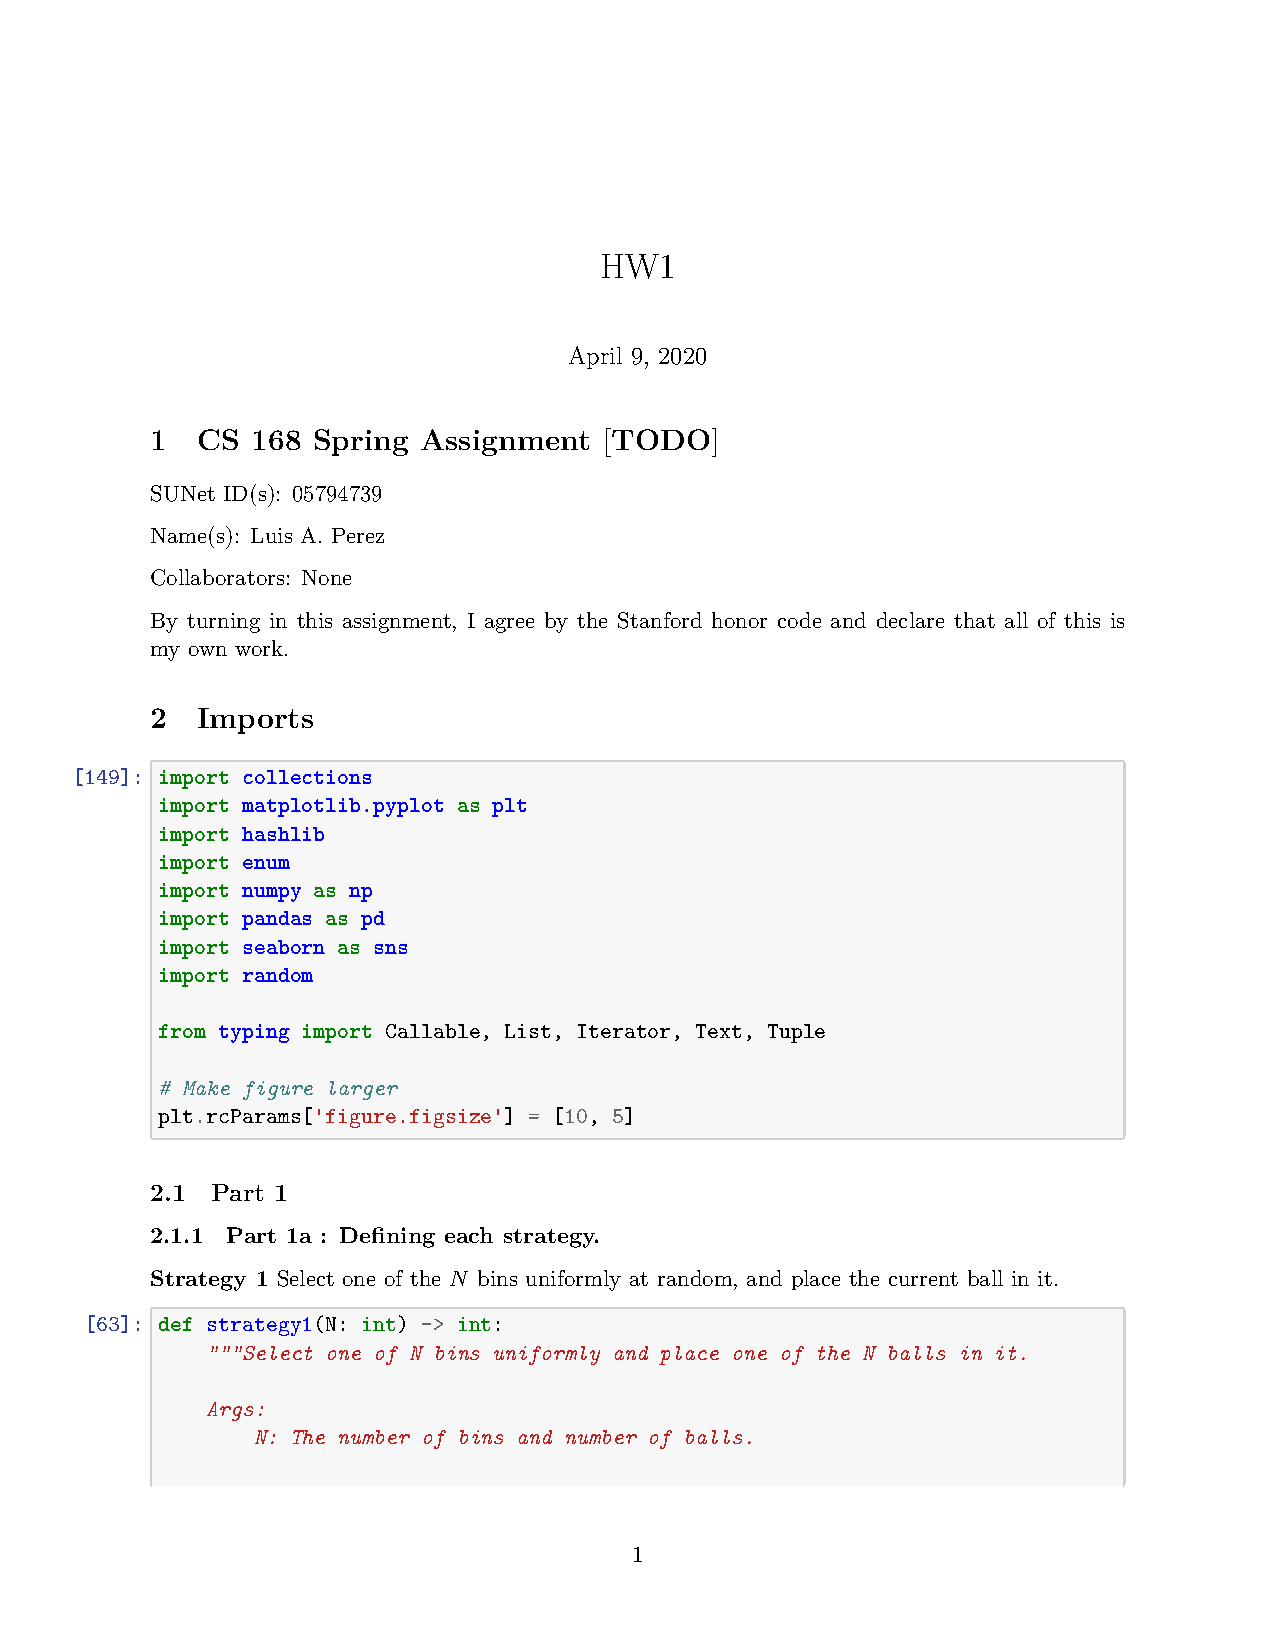
\includepdf[pages=-]{HW1}



\end{document}
